% Copyright (C)  2018  TANSORIER.
% Permission is granted to copy, distribute and/or modify this document
% under the terms of the GNU Free Documentation License, Version 1.3
% or any later version published by the Free Software Foundation;
% with no Invariant Sections, no Front-Cover Texts, and no Back-Cover Texts.
% A copy of the license is included in the section entitled "GNU
% Free Documentation License".

% https://www.gnu.org/licenses/fdl-1.3.html

% compress option to have horyzontal circle
\documentclass[aspectratio=169]{beamer}

%%%%%%%%%%%%%%%%%%%%%%%%%%%%%%%%%%%%%%%%%%%%%%%%%%%%%%%%%%%%%%%%%%%%%

% Thèmes
\usetheme{Darmstadt}

% Redéfini la couleur de base du document
\definecolor{cvp}{RGB}{179,0,161}
\setbeamercolor*{structure}{fg=cvp}

% Language
\usepackage[french]{babel}

% Pour les hyperliens
\usepackage{hyperref}

%%%%%%%%%%%%%%%%%%%%%%%%%%%%%%%%%%%%%%%%%%%%%%%%%%%%%%%%%%%%%%%%%%%%%
\title[U-Boot]{Café Vie Privée \\ \textbf{Alternative pour Android}}
\titlegraphic{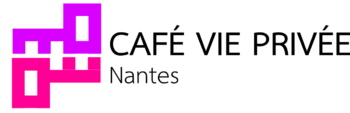
\includegraphics[width=.5\textwidth]{logos/CVP-Nantes.png}}

\author[Café Vie Privée]{Café Vie Privée}

\date[Août 2018]{\textit{Présentation d'outils libres pour se protéger sur Android}}
%%%%%%%%%%%%%%%%%%%%%%%%%%%%%%%%%%%%%%%%%%%%%%%%%%%%%%%%%%%%%%%%%%%%%

% Pour enregistrer l'écran
% ========================
% (activer le debugage par usb pour accèder vie adb)
% adb shell screenrecord --output-format=h264 - | ffplay -

\begin{document}

% *******************************
% ****     PAGE DE GARDE     ****
% *******************************

\begin{frame}
\titlepage
\end{frame}

% Ajout le logo sur les diapos après la page de garde
\logo{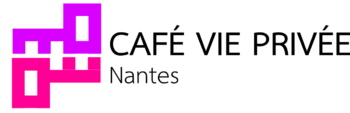
\includegraphics[width=.20\textwidth]{logos/CVP-Nantes.png}}

% *******************************
% ****      INTRODUCTION     ****
% *******************************

\begin{frame}{Déroulé}
\tableofcontents[hideallsubsections]
\end{frame}

\section{Pourquoi se protéger ?}

\begin{frame}
\begin{center}
\huge{\color{cvp}{Pourquoi se protéger ?}}
\end{center}
\end{frame}

\subsection{Qu'est-ce que Android}

\begin{frame}{}
\begin{block}{Wikipedia}
	\emph{\href{https://fr.wikipedia.org/wiki/Android}{Android}} est un système d'exploitation mobile fondé sur le noyau Linux et développé actuellement par Google.
\end{block}
Android à été lancé en 2007.\newline
Le code est sous \emph{licence apache (ASL)}. Il peut donc être intégré dans des applications propriétaires.
\end{frame}

\begin{frame}{Quelques infos}
On peut le trouver sur
\begin{itemize}
	\item Téléphone
	\item Tablette
	\item Télévision
	\item Livre électronique (ex: chomebook)
	\item Montre
	\item Voiture
	\item …
\end{itemize}
Il possède plus de 80\% de part de marché des smartphone (en 2015).
\end{frame}

\subsection{Économie de la surveillance}

\begin{frame}
\begin{center}
\large{\color{cvp}{Économie de la surveillance}}
\end{center}
\end{frame}

\begin{frame}{Les Publicitaires}
Les applications dépendent d'un model économique, qui souvent est dépendant des publicitaires.\newline
\newline
Pour cela ils utilisent des \texttt{pisteurs}.
\end{frame}

\begin{frame}{Exodus Privacy}
\begin{block}{Exodus Privacy}
Est une plate-forme d'analyse des applications Android qui liste les traqueurs et les autorisations de celles-ci.
\end{block}
Créer en 2017.\newline
\newline
\newline
\textcolor{gray}{\tiny{(ClassyShark3xodus le fait pour les apk de F-droid)}}
\end{frame}

\subsection{Programme de surveillance}

\begin{frame}
\begin{center}
\large{\color{cvp}{Programme de surveillance}}
\end{center}
\end{frame}

\begin{frame}{Les enjeux}
Il existe de nombreux programmes de surveillance plus ou moins connus.
\begin{block}{Jérémy Zimmermamn}
Ne pas confondre entre: j'ai rien à me reprocher et j'ai rien à cacher.
\end{block}
Cf. Lo documentaire Notiong To Hide
\end{frame}

\begin{frame}{}
Refuser les programmes de surveillance des données comme PRISM, XKeyscore et Tempora.
% PRISM: Progamme de surveillanc américan. Collecte les données sur internet.
%	https://fr.wikipedia.org/wiki/PRISM_(programme_de_surveillance)
% XKeyscore: Programme de surveillance créer par la NSA. Collecte quasi systématique des activités de tout utilisateur sur Internet.
%            Révélé en juillet 2013.
% 	https://fr.wikipedia.org/wiki/XKeyscore
% Tempora: Programme britanique permettant d'intercepter les données transitant par les câbles en fibre optique entre l'europe et les États-Unis.

\begin{tiny}
\begin{block}{PRISM}
Progamme de surveillance américan créer par la NSA. Collecte les données sur internet.
Edward Snowden a dénoncé ce programme en juin 2013.
\end{block}

\begin{block}{XKeyscore}
Programme de surveillance créé par la NSA. Collecte quasi systématique des activités de tout utilisateur sur Internet. Révélé en juillet 2013.
\end{block}

\begin{block}{Tempora}
Programme britanique permettant d'intercepter les données transitant par les câbles en fibre optique 	entre l'europe et les États-Unis.
\end{block}
\end{tiny}
\end{frame}

\begin{frame}{Contre attaque}
Il existe des projet pour se défendre contre ça:
\url{https://prism-break.org/fr/categories/android/}\newline
\newline
On y reviendra :)
\end{frame}

\subsection{La surveillance de masse}

\begin{frame}
\begin{center}
\large{\color{cvp}{La surveillance de masse}}
\end{center}
\end{frame}

\begin{frame}{Les puissants - la centralisation}
Nos environnements informatiques utilisent des \textbf{logiciels propriétaires},\newline
et pour la plupart détenue par quelques uns qui ont un \textbf{poids important} dans notre société. \newline
\newline
D'où la création du terme \textbf{GAFAM}: Google Apple Facebook Amazon Microsoft
\end{frame}

\begin{frame}{Les besoins}
Accéder au code source permet d'\textbf{auditer} le code et vérifier que le logiciel correspond à ce pourquoi il est fait. \newline
\newline
Le logiciel libre permet de \textbf{modifier} le code pour nos besoins personnels.\newline
\newline
Ainsi que la \textbf{décentralisation}.
\end{frame}


% *******************************
% ****  COMMENT SE PROTEGER  ****
% *******************************

\section{Comment se protéger ?}

\begin{frame}
\begin{center}
\huge{\color{cvp}{Comment se protéger ?}}
\end{center}
\end{frame}

\begin{frame}
En utilisant du logiciel Libre.\newline
On se permet d'auditer le code source,\newline
de l'adapter pour soi même.\newline
Donc il ne \textbf{dépend pas} d'un \textbf{modèle économique} particulier.
\end{frame}

\subsection{Avec quels logiciels ?}

\begin{frame}
On va voir quelques exemples:\newline
\begin{itemize}
	\item Magasin d'applications
	\item Navigation
	\item Réseaux sociaux
	\item Cartes
	\item Multimédia
	\item Recherches
	\item Divers
\end{itemize}
\end{frame}


% *******************************
% ****   LES APPLICATIONS    ****
% *******************************

\section{Les Applications}

\begin{frame}
\begin{center}
\huge{\color{cvp}{Les Applications}}
\end{center}
\end{frame}

\subsection{Magasin d'application}

\begin{frame}
Playstore $\to$ F-Droid\newline
Playstore $\to$ Aurora Droid\newline
\newline
Playstore $\to$ Yalp store\newline
Playstore $\to$ Aurora Store
\end{frame}

\subsection{Navigation}
\begin{frame}
Chrome $\to$ Firefox\newline
Google $\to$ Duckduckgo\newline
\newline
Tor Browser \textcolor{gray}{\tiny{(anciennement Orfox)}}\newline
\newline
Orobot \textcolor{gray}{\tiny{(Proxy pour le réseau Tor)}}
\end{frame}

\subsection{Réseaux sociaux}
\begin{frame}
Facebook $\to$ slim social \textcolor{gray}{\tiny{(ou Frost for fackbook)}}\newline
\newline
Diaspora\newline
Mastodon
\end{frame}

\subsection{Messagerie instantanée}
\begin{frame}
Whatsapp $\to$ Signal\newline
SMS $\to$ Silence\newline
Conversation \textcolor{gray}{\tiny{(XMPP)}}
\end{frame}

\subsection{Cartes}
\begin{frame}
OsmAnd \textcolor{gray}{\tiny{(Openstreetmaps)}}
\end{frame}

\subsection{multimédia}
\begin{frame}
Youtube $\to$ NewPipe\newline
Peertube $\to$ Thoruim
\end{frame}

\subsection{Recheche}
\begin{frame}
Google $\to$ Duckduckgo
\end{frame}

\subsection{Divers}
\begin{frame}
\begin{description}
	\item[Clavier] Google $\to$ AnySoftKey
	\item[Météo] Votre météo locale \textcolor{gray}{\tiny{(F-droid)}}
	\item[Caméra] Open Caméra
	\item[Transport] Transportr
	\item[Bloqueur] Blokada
	\item[Liseure] Book Reader
	\item[Luminosité] Red Moon
	\item[Battery] Drowser
\end{description}
\end{frame}

% *******************************
% ****     OS ALTERNATIF     ****
% *******************************

\section{OS Alternatif}

\begin{frame}
\begin{center}
\huge{\color{cvp}{OS Alternatif}}
\end{center}
\end{frame}

\subsection{État de l'art}
\begin{frame}
Il n'existe pas beaucoup d'alternatives complètes, car la difficulté est le support matériel du téléphone.

Exemple:
\begin{itemize}
	\item Replicant
	\item PureOS
	\item LineageOS
\end{itemize}
\end{frame}

\subsection{Replicant}
\begin{frame}
\href{https://fr.wikipedia.org/wiki/Replicant_\%28syst\%C3\%A8me_d\%27exploitation\%29}{Replicant} est un système d'exploitation entièrement libre pour les smartphones et les tablettes, en remplaçant les composants privateurs d'Android par leurs équivalents libres.
\end{frame}

\subsection{PureOS}
\begin{frame}
Fait pour \href{https://puri.sm/products/librem-5/}{Librem5}.\newline

\url{https://puri.sm/products/librem-5/pureos-mobile/}
\end{frame}

\subsection{LineageOS}
\begin{frame}
- Théorie avec microG
\end{frame}
\subsection{MicroG}
\begin{frame}
- Avantage du contrôle accès applications
- Démo
\end{frame}

\end{document}
